\chapter{Runway design}

	\section{Declared distances}
		\subsection{Runway 1}
		\paragraph{}The first declared distance that will be calculated is the landing distance. Using the maximum landing weight (251.000kg) which can be found in the ACAP paper and considering standard atmosphere conditions and sea level, the value can be obtained using the graph shown below: 
		
		\begin{figure}[H]
			\centering
			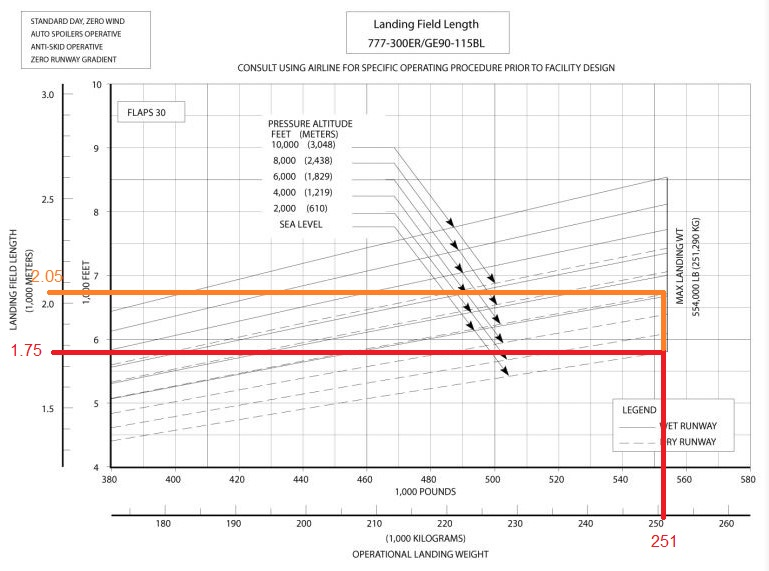
\includegraphics[clip, trim=0cm 0cm 0cm 0cm, width=0.95\textwidth]{./images/B777/landingdistance777}
			\caption{Landing distance vs MTOW for the Boeing 777.} %nom de la figura
			\label{} %per denotar una referencia
		\end{figure}
		
		The landing distance is 1.750m for dry runway and 2.050 for wet runway. Since the runway length is higher than those values, the available landing distance will be equal to the runway length.	Now, increasing its value by a coefficient of 67\%, the final landing distance obtained is 2.920m in dry runways and 3.417m. 
		
		The next distance that will be calculated is the takeoff length without engine failure (TODA). In order to calculate it, the reference field length (3.290m) will be corrected with a factor of 15\%.  The final TODA obtained is 3.783m.
		
		
		Moving into the takeoff length with engine failure (TORA), some hypotheses need to be done in order to calculate the final distance.  Due to the fact that the engine failure occurs after the critical velocity (v1) which is achieved at the 70\% of the runway total length, the thrust coefficient is reduced after that point. The final TORA obtained has a value of 4.120m.
		
		
		Finally, the last declared distance is the Accelerate-Stop Distance Available (ASDA). This distance also requires a hypothesis in order to be solved. The takeoff is cancelled before the critical velocity (v1), thus at the 65\% of the runway length. To compute the final ASDA, the landing distance has to be added to the 65\% of the runway length. The value obtained is 3890m.  
		
		All the declared distances obtained are minimum values, thus, in order to give them a safety margin due to the amount of hypothesis made during the estimation of the values, all the distances have been further increased. 
		
		\subsection{Runway 2}
		\paragraph{}Moving into the second runway, the first declared distance that will be calculated is the landing distance. The value can be obtained using the graph found on the air plane ACAP data-sheet. The maximum landing weight (66.300kg) which can be found in the same paper and considering standard atmosphere conditions and sea level, the value obtained is 1.750m for dry runway and 2.050 for wet runway.
		
		\begin{figure}[H]
			\centering
			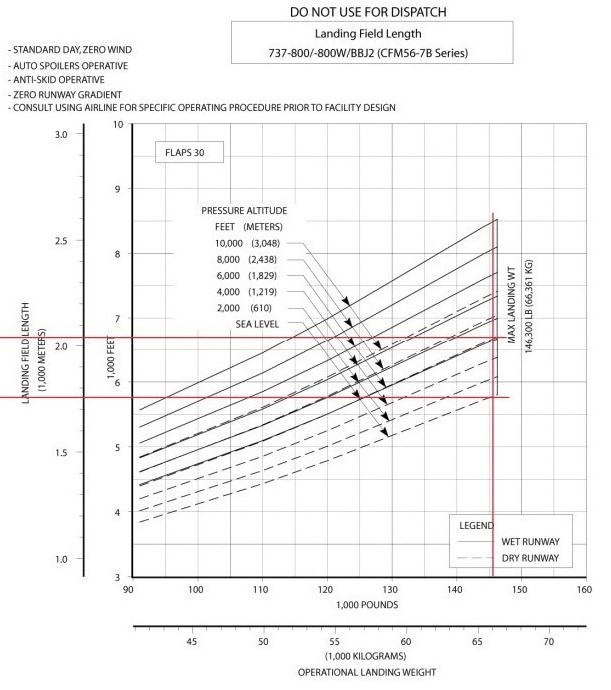
\includegraphics[clip, trim=0cm 0cm 0cm 0cm, width=0.9\textwidth]{./images/B737/landingdistance737}
			\caption{Landing distance vs MTOW for the Boeing 737.}
			\label{} %per denotar una referencia
		\end{figure}
	
	Applying the 67\% safety factor, the values obtained are:  2920m for dry runway and 3423m for wet runway.
	
	The next distance that will be calculated is the takeoff length without engine failure (TORA). The reference field length (2.530m) will be corrected with a factor of 15\%.  The final TORA obtained is 2.750m.
	
	Moving into the takeoff length with engine failure (TODA), some hypotheses need to be done in order to calculate the final distance.  Due to the fact that the engine failure occurs after the critical velocity (v1) which is achieved at the 70\% of the runway total length, the thrust coefficient is reduced after that point. The final TODA obtained has a value of 3.160m.
	
	Finally, the last declared distance is the Accelerate-Stop Distance Available (ASDA). As for the 777, this distance requires a hypothesis in order to be solved. The takeoff is cancelled before the critical velocity (v1), thus at the 65\% of the runway length. To compute the final ASDA, the landing distance has to be added to the 65\% of the runway length. The value obtained is 3.400m.     
	
	As for the runway 1, the values obtained here are the minimum required, thus, in order to give it a security margin due to the amount of hypothesis made during the calculations, the final values may be increased.
	
	\section{Pavement}
		\subsection{Runway 1}
		\paragraph{}In order to calculate the pavement of the runway, the parameter needed are the following:
	
		- The number of operations per year of the most critical aircraft.  
	
		- The maximum take off weight and landing gear configuration of the critical plane. 
	
		- An estimation of the local ground CBR.
	
		Due to the fact that the Boeing 777 has the maximum gross weight by far and its number of operations is close to a 10\% of the total operation on the runway 1, it has been chosen as the critical aircraft in order to calculate the runway thickness.
	
		The number of operations can be estimated using the prognosis, the maximum gross weight and landing configuration can be obtained form the aircraft's ACAP and the local ground CBR value is estimated to 5. Thus, introducing the number of operations per year, which are 6.500 Op/year approximately, using a gross weight of 750.000lbs and a CBR of 5 and making use of the following graph obtained from the FAA, the value of the maximum thickness (\(T_{t}\)) can be obtained:
	   
		\begin{figure}[H]
			\centering
			\includegraphics[clip, trim=0cm 0cm 0cm 0cm, width=0.85\textwidth]{./images/pavement/B777/thickness}
			\caption{Thickness vs gross weight, CBR and operations per year.}
			\label{} %per denotar una referencia
		\end{figure}
	
		As it is stated on the figure, the  value of thickness obtained is 48in, which are 122cm. 
		
		Now, the next step is to calculate the thickness that will have the first two layers. In order to do that, the same graph will be used. However, this time, the CBR of the cement will be considered 25. 
		
		\begin{figure}[H]
			\centering
			\includegraphics[clip, trim=0cm 0cm 0cm 0cm, width=0.85\textwidth]{./images/pavement/B777/thickness2}
			\caption{Thickness of the two first layers vs gross weight, CBR and operations per year.}
			\label{} %per denotar una referencia
		\end{figure}
		
		The value obtained is 14in which are 36cm. Considering a first layer (\(T_1\)) of 13cm, the thickness of the second layer (\(T_2\)) will be 23cm. Before considering the results as valid, a testing of the minimum thickness of (\(T_1\)) and (\(T_2\)) has to be done according to the FAA. To do so, the graph shown above must be followed:
		
		\begin{figure}[H]
			\centering
			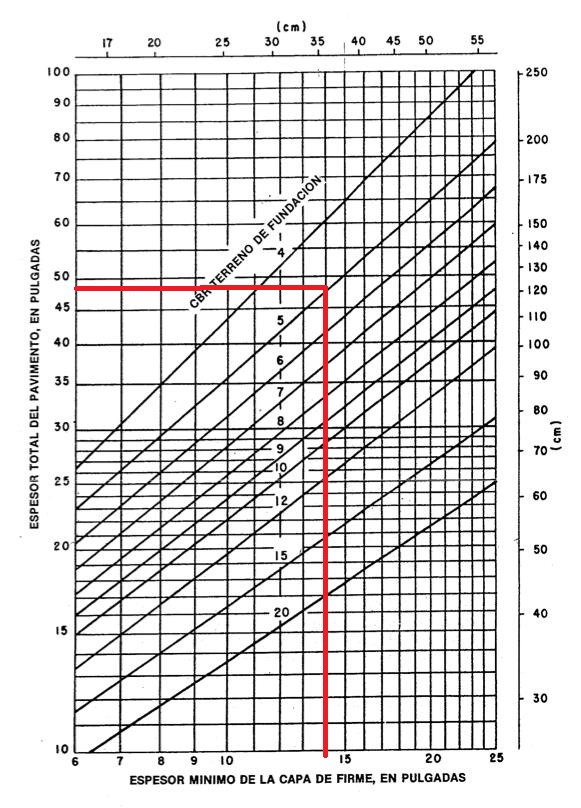
\includegraphics[clip, trim=0cm 0cm 0cm 0cm, width=0.65\textwidth]{./images/pavement/B777/thicknes2min}
			\caption{Minimum thickness of the two first layers vs total thickness.}
			\label{} %per denotar una referencia
		\end{figure}
	
		As it can be seen, entering the maximum thickness and the estimated CBR, the value of 14in for the first two layers is obtained. That exactly the same value that we had calculated using the other graph method, thus, the thickness of the first two layers is correct.
	
		Moving on to the calculation of the last layer (\(T_3\)), it can be easily done by once the other 3 thickness are known. 
		
		\[T_3 = T_t - T_1 - T_2 = 122 - 23 - 13 = 86cm\]
		
		The final value obtained is 86cm. Now, the next step is to consider each material used on the cement and firms using the following tables extracted form the FAA:
		
		\begin{figure}[H]
			\centering
			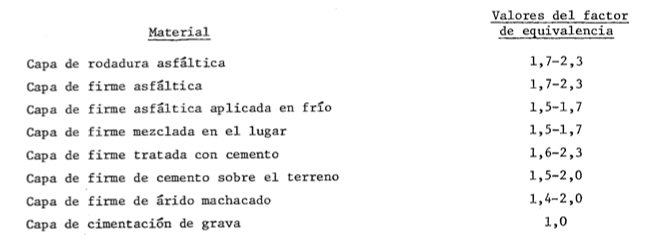
\includegraphics[clip, trim=0cm 0cm 0cm 0cm, width=1\textwidth]{./images/pavement/cemento}
			\caption{Cement materials and their equivalence factor.}
			\label{} %per denotar una referencia
		\end{figure}
	
		\begin{figure}[H]
			\centering
			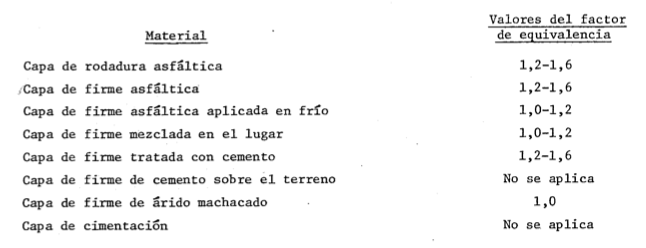
\includegraphics[clip, trim=0cm 0cm 0cm 0cm, width=1\textwidth]{./images/pavement/firmes}
			\caption{Firm materials and their equivalence factor.}
			\label{} %per denotar una referencia
		\end{figure}
		
		The materials and values of equivalence chosen are:
		
		- Firm asphalt with a value of 1,1.
		
		- Crushed arid in cement with a value of 1,4.
		
		The next step is to divide the thickness of the \(T_2\) by 1,1 and the thickness \(T_3\) by 1,4. The minimum values have been chosen in order to maximise the security factor of the runway. 
		
		The final values obtained will be displayed on the table below:
		
		\begin{table}[htb]
			\centering
			\begin{tabular}{ll p{5cm}}
				\midrule[2pt]
				\(T_1\)& 13 cm\\
				\(T_2\) & 21 cm\\
				\(T_3\)& 62 cm \\
				\(T_t\)& 95 cm\\
				\bottomrule[2pt]
			\end{tabular}
			\caption{Thickness after the materials correction factor.}
			\label{}
		\end{table}
		
		However, the values obtained form correcting the thickness with the materials is not enough, there is still one more correction to be done, the one regarding the number of operations per year. To do that, the maximum number of operations per year stated on the prognosis will help us to solve the following equation:
		\[T_{total} = T_t * (1+0,133*\log(\dfrac{N}{25.000})) = 95 * (1+0,133*\log(\dfrac{135.000}{25.000}))= 104,5cm\]
		
		Finally, the total thickness is obtained with a value of 104,5cm. The last step is to distribute the increase of thickness between the three layers. The final thickness of each layer will be the following:
		
		\begin{table}[htb]
			\centering
			\begin{tabular}{ll p{5cm}}
				\midrule[2pt]
				\(T_1\)& 14 cm\\
				\(T_2\) & 25 cm\\
				\(T_3\)& 65,5 cm \\
				\(T_t\)& 104,5 cm\\
				\bottomrule[2pt]
			\end{tabular}
			\caption{Final values of thickness of each layer.}
			\label{}
		\end{table}
		
		\subsection{Runway 2}
		\paragraph{}As for the runway1, the same parameters are needed in order to calculate the thickness od the second runway. In this case, the critical aircraft is the Boeing 737 due to its high MTOW and its huge number of operations on the domestic runway.
		
		The number of operations can be estimated using the prognosis, the maximum gross weight and landing configuration can be obtained form the aircraft's ACAP and the local ground CBR value is estimated to 5, like in runway 1. Thus, introducing the number of operations per year, which are 20.000 Op/year approximately, using a gross weight of 160.000lbs and a CBR of 5 and making use of the following graph obtained from the FAA, the value of the maximum thickness (\(T_{t}\)) can be obtained:
		
		\begin{figure}[H]
			\centering
			\includegraphics[clip, trim=0cm 0cm 0cm 0cm, width=0.85\textwidth]{./images/pavement/B737/thickness}
			\caption{Thickness vs gross weight, CBR and operations per year.}
			\label{} %per denotar una referencia
		\end{figure}
		
		As it is stated on the figure, the  value of thickness obtained is 40in, which are 102cm. 
		
		Now, the next step is to calculate the thickness that will have the first two layers. In order to do that, the same graph will be used. However, this time, the CBR of the cement will be considered 25. 
		
		\begin{figure}[H]
			\centering
			\includegraphics[clip, trim=0cm 0cm 0cm 0cm, width=0.85\textwidth]{./images/pavement/B737/thickness2}
			\caption{Thickness of the two first layers vs gross weight, CBR and operations per year.}
			\label{} %per denotar una referencia
		\end{figure}
		
		The value obtained is 14in which are 36cm. Considering a first layer (\(T_1\)) of 12cm, the thickness of the second layer (\(T_2\)) will be 24cm. Before considering the results as valid, a testing of the minimum thickness of (\(T_1\)) and (\(T_2\)) has to be done according to the FAA. To do so, the graph shown above must be followed:
		
		\begin{figure}[H]
			\centering
			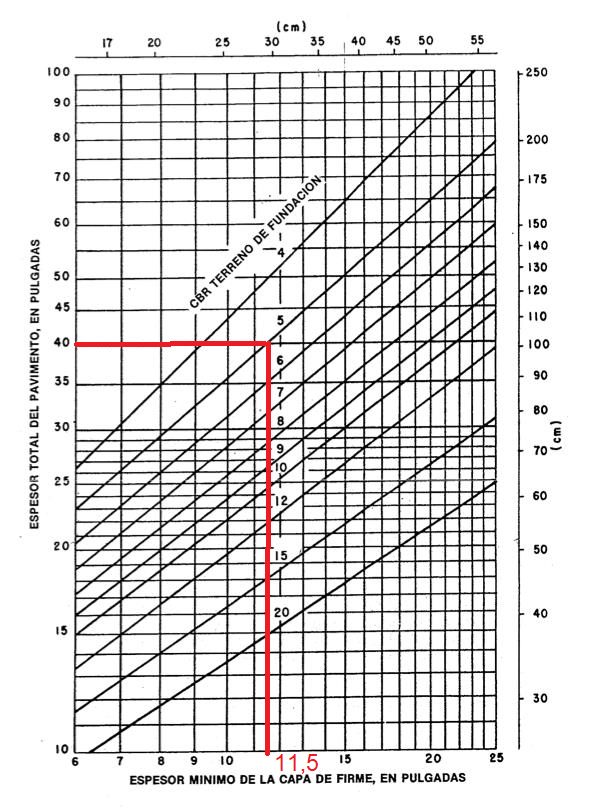
\includegraphics[clip, trim=0cm 0cm 0cm 0cm, width=0.65\textwidth]{./images/pavement/B737/thickness2min}
			\caption{Minimum thickness of the two first layers vs total thickness.}
			\label{} %per denotar una referencia
		\end{figure}
		
		As it can be seen, entering the maximum thickness and the estimated CBR, the minimum value of 11,5in for the first two layers is obtained. Due to the fact that the thickness obtained by the other method has a value of 14in, the result is considered valid since its value is greater than the minimum required by the FAA.
		
		Moving on to the calculation of the last layer (\(T_3\)), it can be easily done by once the other 3 thickness are known. 
		
		\[T_3 = T_t - T_1 - T_2 = 102 - 24 - 12 = 66cm\]
		
		The final value obtained is 66cm. Now, the next step is to consider each material used on the cement and firms using the following tables extracted form the FAA:
		
		\begin{figure}[H]
			\centering
			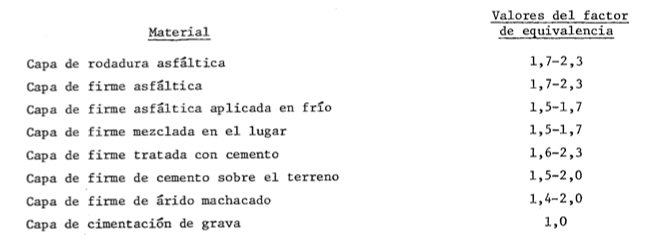
\includegraphics[clip, trim=0cm 0cm 0cm 0cm, width=1\textwidth]{./images/pavement/cemento}
			\caption{Cement materials and their equivalence factor.}
			\label{} %per denotar una referencia
		\end{figure}
		
		\begin{figure}[H]
			\centering
			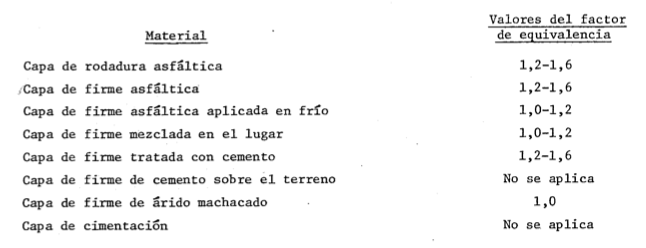
\includegraphics[clip, trim=0cm 0cm 0cm 0cm, width=1\textwidth]{./images/pavement/firmes}
			\caption{Firm materials and their equivalence factor.}
			\label{} %per denotar una referencia
		\end{figure}
		
		The materials and values of equivalence chosen will be the same as for runway 1 in order to ease the construction of the runway process. Thus:
		
		- Firm asphalt with a value of 1,1.
		
		- Crushed arid in cement with a value of 1,4.
		
		Dividing the thickness of the \(T_2\) by 1,1 and the thickness \(T_3\) by 1,4, the values obtained after the materials correction are:
		
		\begin{table}[htb]
			\centering
			\begin{tabular}{ll p{5cm}}
				\midrule[2pt]
				\(T_1\)& 12 cm\\
				\(T_2\) & 21 cm\\
				\(T_3\)& 47 cm \\
				\(T_t\)& 81 cm\\
				\bottomrule[2pt]
			\end{tabular}
			\caption{Thickness after the materials correction factor.}
		\end{table}
		
		\paragraph{}
		
		However, the values obtained form correcting the thickness with the materials is not enough, there is still one more correction to be done, the one regarding the number of operations per year. To do that, the maximum number of operations per year stated on the prognosis will help us to solve the following equation:
		
		\[T_{total} = T_t * (1+0,133*\log(\dfrac{N}{25.000})) = 81 * (1+0,133*\log(\dfrac{270.000}{25.000}))= 91,5cm\]
		
		Finally, the total thickness is obtained with a value of 91,5cm. The last step is to distribute the increase of thickness between the three layers. The final thickness of each layer will be the following:
		
		\begin{table}[htb]
			\centering
			\begin{tabular}{ll p{5cm}}
				\midrule[2pt]
				\(T_1\)& 13 cm\\
				\(T_2\) & 23 cm\\
				\(T_3\)& 55,5 cm \\
				\(T_t\)& 91,5 cm\\
				\bottomrule[2pt]
			\end{tabular}
			\caption{Final values of thickness of each layer.}
			\label{}
		\end{table}
		
		
		
	
	